\documentclass[11pt]{article}
\usepackage[a4paper,margin=21mm]{geometry}
\usepackage[no-math]{fontspec}
\setmainfont{Latin Modern Roman}
\newfontfamily\CJKfont{Noto Serif CJK SC}
\XeTeXlinebreaklocale "zh"
\XeTeXlinebreakskip=0pt plus 1pt
\usepackage{amsmath,amssymb,amsthm,amscd,graphicx,color}
\usepackage{xurl}
\usepackage[unicode,hidelinks]{hyperref}
\allowdisplaybreaks
\setlength\emergencystretch{3em}
\numberwithin{equation}{section}

\usepackage{enumerate}

\numberwithin{equation}{section}

\newtheorem{Theorem}{Theorem}[section]
\newtheorem{Lemma}[Theorem]{Lemma}
\newtheorem{Fact}[Theorem]{Fact}
\newtheorem{Cor}[Theorem]{Corollary}
\newtheorem{Prop}[Theorem]{Proposition}
\newtheorem{State}[Theorem]{Statement}

 { \theoremstyle{definition}
\newtheorem{Definition}[Theorem]{Definition}
\newtheorem{Remark}[Theorem]{Remark} }

\def\II{{\rm II}}
\def\tr{{\rm tr}}

\def\A{\mathbb{A}}
\def\R{\mathbb{R}}
\def\B{\mathbb{B}}
\def\S{\mathbb{S}}
\def\H{\mathbb{H}}
\def\T{\mathbb{T}}
\def\Z{\mathbb{Z}}
\def\C{\mathbb{C}}
\def\D{\mathbb{D}}

\def\Bb{\mathbf{B}}

\def\bs{\boldsymbol}

\def\zerob{\mathbf{0}}
%\def\zerob{O}

\def\RP{\mathbb{RP}}
\def\refOmega{\Omega_0}

\def\Ucal{\mathcal{U}}
\def\Lcal{\mathcal{L}}
\def\Hcal{\mathcal{H}}
\def\Acal{\mathcal{A}}
\def\Ccal{\mathcal{C}}
\def\Dcal{\mathcal{D}}
\def\Pcal{\mathcal{P}}
\def\Ical{\mathcal{I}}
\def\Bcal{\mathcal{B}}
\def\Scal{\mathcal{S}}
\def\Ecal{\mathcal{E}}
\def\Tcal{\mathcal{T}}
\def\Zcal{\mathcal{Z}}
\def\Ncal{\mathcal{N}}
\def\Qcal{\mathcal{Q}}
\def\Ocal{\mathcal{O}}
\def\Xcal{\mathcal{X}}
\def\Zcal{\mathcal{Z}}
\def\Vcal{\mathcal{V}}
\def\Kcal{\mathcal{K}}

\def\Crm{{\rm C}}

\def\Rscr{\mathscr{R}}
\def\Bscr{\mathscr{B}}

\def\nb{{\boldsymbol{n}}}
\def\vb{{\boldsymbol{v}}}
\def\pb{{\boldsymbol{p}}}
\def\ub{{\boldsymbol{u}}}
\def\xb{{\boldsymbol{x}}}

\def\supp{\operatorname{supp}}

\def\ed{{\rm d}}
\def\std{{\rm std}}
\def\Ric{{\rm Ric}}
\def\area{{\rm area}}
\def\length{{\rm length}}
\def\Hess{{\rm Hess}}
\def\vol{{\rm vol}}
\def\dvol{{\;d\rm vol}}
\def\id{{\rm id}}
\def\Rm{{\rm Rm}}
\def\tr{{\rm tr}}
\def\div{{\rm div}}
\def\sec{{\rm sec}}
\def\width{{\rm width}}
\def\Lip{{\rm Lip}}
\def\dist{{\rm dist}}
\def\pt{{\rm pt}}
\def\inj{{\rm inj}}
\def\exp{{\rm exp}}
\def\rank{{\rm rank\;}}
\def\const{{\rm const}}
\def\sys{{\rm sys}}
\def\loc{{\rm loc}}
\def\Rm{{\rm Rm}}
\def\tilRm{\widetilde\Rm}

\def\nub{\boldsymbol{\nu}}
\def\cmc{\mu}

\def\<{\langle}
\def\>{\rangle}

\def\hemiN{\S^n_+}
\def\hemiT{\S^3_+}

\def\setdiff{\backslash}

\def\Nsep{\textbf{\textup{NSep}$^+$}}

\begin{document}
\begin{center}\Large Compact-region nonhyperbolic deformations of Hn/Z\textasciicircum{}(n-2) preserving the hyperbolic scalar-curvature lower bound in every dimension n>=3\end{center}
\noindent\textbf{Stable ID:} 1168\quad\textbf{Author:} Tianze Hao; Yuhao Hu; Peng Liu; Yuguang Shi\par
\noindent\textbf{Work:} Rigidity and Non-Rigidity of $\mathbb{H}^n/\mathbb{Z}^{n-2}$ with Scalar Curvature Bounded from Below\par
\noindent\textbf{Source:} \url{https://sigma-journal.com/2023/083/}\par
\noindent\textbf{Version:} Official SIGMA 19 (2023) article 083, DOI 10.3842/SIGMA.2023.083; journal PDF and native TeX acquired 2026-09-30, exact bytes pinned by SHA256\par
\noindent\textbf{Rights:} CC BY 4.0. Authors retain copyright. \url{https://creativecommons.org/licenses/by/4.0/}. Reuse and typesetting adaptation; original language and mathematical content preserved.\par
\noindent\textbf{Difficulty (prior selection preserved):} {\CJKfont H2: The construction matches two distinct warped-product boundary geometries while making the replacement scalar curvature and mean curvature sufficiently large. It modifies the hyperbolic collar by a flat-ended radial factor whose derivative supplies a strict scalar-curvature margin. That margin absorbs the smoothing loss in the gluing theorem, producing a complete nonhyperbolic metric with an exactly unchanged exterior and the sharp lower bound.}\par
\medskip\noindent\textbf{Editorial boundary note (not author text):} Complete original independent non-rigidity Theorem1.2 for all n>=3 and full Section2.1–2.3 author construction. The exact standard parabolic lattice quotient/exterior interpretation, both warped boundary geometries and their coordinate/mean/scalar-curvature estimates, replacement metric and boundary isometry, corner-smoothing assumptions, full flat-ended radial collar/strict scalar margin, Fermi identification and absorption of the epsilon loss are retained. The author explicitly marks the displayed coordinate-gradient/Hessian formulas as standard computations; their exact inputs/formulas remain present without editor verification. The published smoothing theorem and stated standard warped scalar-curvature identity are precise formal prerequisites. Original Figure1 schematic is unchanged with every printed region/metric/curvature/coordinate label separately editable and asset-bound. One independent construction, expressly said to be technically independent of the rest; later topology-preserving refinements, rigidity and splitting results are excluded. The original theorem asserts existence of a complete manifold with an unchanged exterior, not a prescribed global topology; the statement and all literal signs/coordinates are preserved.\par
\medskip\hrule\medskip\noindent\textbf{Author text begins below.}\par

% Original source lines 167--192
\section{Introduction}

In \cite[Section 3]{Gr2019} and \cite[p.~240]{Gr2021}, Gromov stated the following generalization
of Min-Oo's hyperbolic rigidity theorem \cite{MinOo89}.

\begin{State}[``generalised Min-Oo rigidity theorem'']\label{generminoo}
Parabolic quotients $Z=\mathbb{H}^n/\Gamma$ of the hyperbolic $n$-space admit no non-trivial, compactly supported `deformation' with scalar curvature $R\geq -n(n-1)$.
\end{State}
According to \cite{Gr2019}, a \emph{deformation} can change not only the metric, but also the topology of a compact region in $Z$.
If the deformation is topologically a connected sum with
a closed $n$-manifold,
Statement~\ref{generminoo} is known to be true for (at least) $Z = \H^n/\Z^{n-1}$,
with idea of proof already outlined by \cite[Section $5\frac{5}{6}$]{Gr93} (for a detailed treatment, see
also  \cite[Theorem 1.1]{ACG08}).
The situation
turns out to be more subtle
if broader types of deformations are considered, allowing, for example, surgeries along
an embedded, non-contractible loop.
In this latter case we construct a counterexample to Statement~\ref{generminoo}, which, more precisely,
demonstrates the following.

\begin{Theorem}\label{counterexample}
For $n\ge 3$, let $\mathbb{H}^n/\mathbb{Z}^{n-2}$ be equipped with the standard hyperbolic metric.
There exists a complete Riemannian manifold $(M^n,g)$, not $($globally$)$ hyperbolic, and
compact subsets $K\subset M$ and $K'\subset\H^n/\Z^{n-2}$, such that $(1)$~$R_g\ge -n(n-1)$ and $(2)$~$M\setminus K$ is isometric to~$\big(\mathbb{H}^n/\mathbb{Z}^{n-2}\big)\setminus K'$.	
\end{Theorem}


% Original source lines 402--755
\section[Non-rigidity of H\^{}n/Z\^{}(n-2)]{Non-rigidity of $\boldsymbol{\H^n/\Z^{n-2}}$}\label{Non-rigidity}

Let the hyperbolic $n$-space $\H^n$ be represented by the upper half-space model
$\R^n_+ = \{(x,\boldsymbol{y},z)$: $x\in \R, \boldsymbol{y}\in \R^{n-2}, z>0\}$,
and let $\Z^{n-2}$ act by translating along the orthogonal lattice $2\pi \Z^{n-2}\subset \R^{n-2}$
while keeping the $x,z$-coordinates fixed. The quotient space is denoted by
$\H^{n}/\Z^{n-2}$ and has the hyperbolic metric
\begin{equation}\label{gHdef}
	g_{H} = z^{-2}\bigl(\ed z^2 + \ed x^2\bigr) + z^{-2} g_{\T^{n-2}},
\end{equation}
where the subscript `$H$' stands for `hyperbolic', and $g_{\T^{n-2}}$ is the associated flat metric on~$\T^{n-2}$.
Henceforth, we will regard $(x,z)$ as coordinates on the hyperbolic plane $\H^2$;
manifestly that $\big(\H^{n}/\Z^{n-2},g_H\big)$ is a warped product of $\H^2$ and $\big(\T^{n-2}, g_{\T^{n-2}}\big)$.

The following lemma is easily verified by standard computation, so we omit its proof.
\begin{Lemma}\label{H2DerHess}
Let $\nabla$, $\nabla^2$ denote the gradient and Hessian
with respect to $g_H$ (same below). We~have
\begin{enumerate}\itemsep=0pt
    \item[$(a)$] $\nabla z=z^2{\partial}/{\partial z}$,
	\item[$(b)$] $\nabla^2z({\partial}/{\partial x}, {\partial}/{\partial x}) = -\nabla^2z({\partial}/{\partial z}, {\partial}/{\partial z})=-1/z$,
    \item[$(c)$] $\nabla^2z({\partial}/{\partial z}, {\partial}/{\partial x})=0$.
\end{enumerate}	
\end{Lemma}

Next, we proceed to prove
Theorem~\ref{counterexample} by constructing an example
that satisfies all its conditions. The idea is to remove a suitable compact
subset, $X_{p,r}$, from $\H^n/\Z^{n-2}$ and then `glue' the result with a
compact manifold, $\bar X_r$, along their boundaries; $X_{p,r}$ and
$\bar X_r$ will be defined in Sections~\ref{1stprelimSec} and \ref{2ndprelimSec}
respectively, and then we handle the gluing step
in Section~\ref{gluingSec}.






\subsection{First preliminary construction}\label{1stprelimSec}
Let $p\in \H^2$, and define
\begin{equation}\label{Xrp_def}
	X_{p,r}:= \D_r(p)\times \T^{n-2}\subset \H^{n}/\Z^{n-2} \qquad
	\mbox{and} \qquad  Y_{p,r} :=\partial X_{p,r},
\end{equation}
where $\D_r(p)\subset \H^2$ is the geodesic disc, centered at $p$, of radius $r>0$;
the inclusion in \eqref{Xrp_def} makes sense since $\H^n/\Z^{n-2}$ is a warped product
of $\H^2$ and $\T^{n-2}$, as we already noted.

Now we have two sets of coordinates for $\H^2$: $(x,z)$ and the polar coordinates
$(\varrho,\theta)$ centered at $p$. In terms of the polar coordinates, the metric on $\H^2$ reads
\begin{equation*}%\label{H2metricpolar}
	g_{\H^2} = \ed\varrho^2 + \sinh^2\varrho\,\ed\theta^2.
\end{equation*}



\begin{Lemma}\label{YprMean}
The boundary $Y_{p,r}\subset (X_{p,r}, g_H)$ has the mean curvature
\begin{equation}\label{Hpr}
	H_{p,r}=\coth r-(n-2)z^{-1}\frac{\partial z}{\partial \varrho}.
\end{equation}
Moreover,
\begin{enumerate}\itemsep=0pt
    \item[$(a)$] $|H_{p,r} - \coth r| \leq n-2$;
	\item[$(b)$] There exists a constant $r_0>0$ such that $H_{p,r}>0$ for all $r\leq r_0$.
\end{enumerate}

\end{Lemma}
\begin{proof}
The formula \eqref{Hpr} is straightforward to check by using the representation
\[
	g_H = \ed\varrho^2 + \sinh^2\varrho\,\ed\theta^2 + z^{-2}g_{\T^{n-2}}.
\]
Moreover, since both $z^{-1}\nabla z$ and $\nabla \varrho$ have unit norm with respect to $g_H$,
\begin{equation}\label{dzdrhoBd}
\left|\frac{\partial z}{\partial \varrho}\right|
= \left|\bigl\langle\nabla z, \nabla \varrho \bigr\rangle\right| =\left|z\bigl\langle z^{-1}\nabla z, \nabla \varrho \bigr\rangle\right|\le z.
\end{equation}
This implies $(a)$, and $(b)$ follows since $\coth r\rightarrow\infty$ as
$r\rightarrow 0$.
\end{proof}

\begin{Lemma}\label{dthetazEst}
	There exists a constant $C_r>0$, depending only on $r$, such that on $\partial\D_r(p)$ we have
	\begin{equation*}
		\left|\partial_\theta z (r,\theta)\right| \le z \sinh r \qquad
		\mbox{and}\qquad
		\left|\partial_\theta^2 z(r,\theta)\right| \le C_r z.
	\end{equation*}
\end{Lemma}
\begin{proof}
	Since both $z^{-1}\nabla z$ and $(\sinh r)^{-1}(\partial/\partial\theta)$
	have unit norm with respect to $g_{H}$, we have
	\[
		|\partial_\theta z(r,\theta)| = \left|\bigl\langle\nabla z, \partial/\partial\theta\bigr\rangle\right|
		\le z\sinh r.
	\]
	Moreover, a calculation shows that
	\begin{equation}\label{hessztt}
		\nabla^2 z (\partial/\partial\theta,\partial/\partial\theta)
		= \partial_\theta^2 z  +(\partial_\varrho z) \sinh \varrho \cosh \varrho.
	\end{equation}
	By Lemma~\ref{H2DerHess}\,$(b)$,\,$(c)$, the left-hand side of \eqref{hessztt} has its magnitude bounded
	by $(\sinh^2\rho)z$; thus, using~\eqref{dzdrhoBd} and evaluating
	\eqref{hessztt} at $\varrho = r$, we get
	\[
		\big|\partial_\theta^2 z(r,\theta)\big| \le \sinh r (\sinh r + \cosh r) z.
	\]
	Taking $C_r  = \sinh r(\sinh r + \cosh r)$ finishes the proof.
\end{proof}


\subsection{Second preliminary construction}\label{2ndprelimSec}
Let $\Dcal$ be a $2$-disc with polar coordinates $\bigl(\bar\varrho,\bar\theta\bigr)$, where
\[
	0\le \bar\varrho\le \pi/3 \qquad \mbox{and}\qquad 0\le \bar \theta<2\pi.
\]
Equip $\Dcal$ with the metric
\[
	g_\Dcal = \ed\bar\varrho^2 + 4\sin^2(\bar\varrho/2)\ed\bar\theta^2.
\]
Thus, $(\Dcal, g_\Dcal)$ is isometric to a `cap' in the round sphere of radius $2$.

Now let $r >0$ and $z(\varrho,\theta)$ be as in Section~\ref{1stprelimSec} above. Consider
\begin{equation*}
	\bar X_r := \S^1 \times \Dcal \times \T^{n-3}
\end{equation*}
equipped with the metric
\begin{equation}\label{barg}
\bar g =\sinh^ 2r \,\ed\theta^2 +\bigl(z(r,\theta)\bigr)^{-2} g_\Dcal+\bigl(z(r,\theta)\bigr)^{-2}g_{\T^{n-3}},
\end{equation}
and let $\bar Y_r := \partial \bar X_r$.
By construction, the boundaries $(Y_{p,r}, g_H|_{Y_{p,r}})$ and $\bigl(\bar Y_r, \bar g|_{\bar Y_r}\bigr)$ are isometric under the obvious identification.


\begin{Lemma}%\label{YrMean}	
The boundary $\bar Y_r\subset \bigl(\bar X_r, \bar g\bigr)$ has the mean curvature
\begin{equation}\label{barHr}
\bar H_r=\frac{\sqrt{3}}{2}z(r,\theta).
\end{equation}
\end{Lemma}
\begin{proof}
Standard computation by using \eqref{barg}.
\end{proof}


Regarding the scalar curvature of a warped-product metric,
the following is well-known.

\begin{Lemma}[{cf.~\cite[Proposition 7.33]{GL1983}}]\label{scalarwarp}
Let $\bigl(N^{n-1}, h\bigr)$ be an $(n-1)$-dimensional Riemannian manifold with scalar curvature $R_h$. Given any smooth function $\phi(\theta)$ defined on an
interval $I$ and a constant $a>0$, the warped product metric
$
	g = a^2\ed\theta^2+ \phi(\theta)^2 h
$
defined on $I\times N$ has the scalar curvature
\begin{equation}\label{scalarWarpEq}
R_g=\frac{n-1}{a^2}\left[-2\left(\frac{\phi'}{\phi}\right)'-n\left(\frac{\phi'}{\phi}\right)^2\right]+ \phi^{-2}R_{h}.
\end{equation}
\end{Lemma}

In our case, to compute the scalar curvature of $\bar g$, it suffices to substitute
$h = g_\Dcal + g_{\T^{n-3}}$, $\phi(\theta) = 1/z(r,\theta)$ and $a = \sinh r$ into \eqref{scalarWarpEq}. Noting that
$R_h = 1/2$, we have
\begin{align}
	R_{\bar g}&=(n-1)(\sinh r)^{-2}\bigl\{-2\partial_\theta[z\partial_\theta(1/z)]-n[z\partial_\theta(1/z)]^2\bigr\} + z^{2}/2\nonumber\\
	&=(n-1)(\sinh r)^{-2}\bigl\{2\bigl(\partial_\theta^2 z\bigr)/z-(n+2)[(\partial_\theta z)/z]^2\bigr\}	+ z^{2}/2,\label{Rgbar}
		\end{align}		
where $z$, $\partial_\theta z$ and $\partial_\theta^2 z$ are evaluated at $(r,\theta)$.

Now we are ready to observe the following.

\begin{Prop}\label{XrbarInfo}
For fixed $r>0$, the manifold $(\bar X_r, \bar g)$ satisfies:
\begin{enumerate}\itemsep=0pt
\item[$(a)$]  The scalar curvature
\[
	R_{\bar g}\geq \frac{1}{2}[z(r,\theta)]^2-C_{n,r}
\] for a
constant $C_{n,r}>0$ depending only on $n$ and $r$. In particular, we have
$
R_{\bar g}>-n(n-1)
$
provided that $p\in \H^2$ is chosen to have a large enough $z$-coordinate;

\item[$(b)$] Under the obvious identification $($isometry$)$ between $Y_{p,r}$ and $\bar Y_r$, we have
 $\bar H_r >H_{p,r}$ provided that the $z$-coordinate of $p$ is large enough.
 \end{enumerate}
\end{Prop}

\begin{proof}
	 $(a)$ follows from \eqref{Rgbar} and Lemma~\ref{dthetazEst};
	 $(b)$ follows from Lemma~\ref{YprMean}\,$(a)$ and \eqref{barHr}.
\end{proof}

\subsection{The gluing step}\label{gluingSec}


\begin{Lemma}[{\cite[Theorem 5]{BMN2011}}] \label{bmnthm5}
Let $\Omega$ be a compact $n$-manifold with boundary $\partial\Omega$, and let~$g$ and~$\tilde g$ be two smooth Riemannian metrics on $\Omega$ such that
\begin{enumerate}\itemsep=0pt
\item[$(a)$] $g-\tilde  g=0$ at each point on $\partial\Omega$;
\item[$(b)$] the mean curvatures satisfy $H_{\tilde g}-H_{g}>0$ at each point on $\partial \Omega$.
\end{enumerate}
Then, given any $\epsilon>0$ and any neighborhood $U$ of $\partial \Omega$, there exists a smooth metric $ \hat g$ on $\Omega$ with the following properties:
\begin{enumerate}\itemsep=0pt
    \item[$(1)$] $R_{\hat g} \geq \min\{R_g , R_{\tilde g} \}-\epsilon $ in $\Omega$;
	\item[$(2)$] $\hat g=\tilde g$ in $\Omega\setminus U$;
	\item[$(3)$] $\hat g= g$	in a neighborhood of $\partial\Omega$.
\end{enumerate}
\end{Lemma}
\begin{Remark}
By an arbitrary extension, in Lemma~\ref{bmnthm5} it suffices to assume that $g $ is defined only in a neighborhood of $\partial \Omega$. 	
\end{Remark}

To prove Theorem~\ref{counterexample},
a basic idea is to apply Lemma~\ref{bmnthm5} to obtain a
metric $\hat g$ on $\bar X_r$ which
agrees with $g_H$ in a neighborhood of $\partial \bar X_r\cong \partial X_{p,r}$,
so $\hat g$ extends smoothly into
$\bigl(\H^{n}/\Z^{n-2}\bigr)\setminus X_{p,r}$ by $g_H$.
A compromise is the $\epsilon$-cost to the scalar curvature estimate.
Thus, one would like to have a bit more scalar curvature
to begin with, so that the cost can be absorbed, maintaining the
desired lower bound $R_{\hat g}\ge -n(n-1)$.
This can be achieved by a suitable deformation of
$g_H$ in a neighborhood of $Y_{p,r}\subset \H^{n}/\Z^{n-2}$, as the following lemma
shows.


\begin{Lemma}\label{tradeoffLemma}
Let
\begin{equation}
u(\varrho)=
		\begin{cases}
			1-{\rm e}^{\frac{1}{\varrho-r_0}},& \varrho< r_0, \\
		    1, & \varrho\geq r_0,
		\end{cases}
\end{equation}
and define
\begin{equation*}%\label{metric2}
g_{H}':=\bigl[u(\varrho)\bigr]^2\ed\varrho^2 +\sinh^2 \varrho\, \ed\theta^2 +\bigl[z(\varrho,\theta)\bigr]^{-2} g_{\T^{n-2}}.
\end{equation*}
As long as $r_0>0$ is small enough, we can find $\delta>0$ such that
\[
	R_{g_{H}'} + n(n-1)  >0\qquad \mbox{for }
 \varrho \in [r_0-2\delta, r_0).
\]
\end{Lemma}

\begin{proof}


By \cite[Claim 2.1]{SWW2022}, we have
\begin{equation}\label{hatscalarcurv}
R_{g_H'}=R_{g_H}+\bigl(1-u^{-2}\bigr)(R_{\gamma(\varrho)}-R_{g_H})+2u^{-3}u'(\varrho) H_{p,\varrho},
\end{equation}
where
${\gamma(\varrho)}= \sinh^2 \varrho \,\ed\theta^2 +\bigl[z(\varrho,\theta)\bigr]^{-2}g_{\T^{n-2}}$ and $R_{g_H} = -n(n-1)$.

We want to estimate the right-hand side of formula~\eqref{hatscalarcurv}. To start with, by Lemma~\ref{scalarwarp},
\begin{equation*}%\label{Rgamma}
R_{\gamma(\varrho)}= (n-2) (\sinh \varrho )^{-2}
\big\{2\big(\partial_\theta^2 z\big)/z -(n+1)[(\partial_\theta z)/z]^2\big\}.
\end{equation*}
Thus, by the proof of Lemma~\ref{dthetazEst}, there exists a constant $C_{n,r_0}$,
depending on $n,r_0$ only, such that
\begin{equation}\label{RgammaBd}
|R_{\gamma(\varrho)}|\leq C_{n,r_0}\qquad\mbox{for } \varrho \in [r_0/2, r_0].
\end{equation}
Next, by the definition of $u$, we have, for $\varrho\le r_0$,
\begin{equation}\label{1minusu}
	0\ge 1 - u^{-2} = u^{-2}\bigl(-2 {\rm e}^{\frac{1}{\varrho - r_0}} + {\rm e}^{\frac{2}{\varrho - r_0}}\bigr) \ge - 2u^{-2} {\rm e}^{\frac{1}{\varrho - r_0}} \ge -2u^{-3} {\rm e}^{\frac{1}{\varrho - r_0}} .
\end{equation}
Moreover, for sufficiently small $r_0$, we have
$H_{p,\varrho} \geq 1$ for any $\varrho\le r_0$ (Lemma~\ref{YprMean}\,$(b)$), and so
\begin{equation}\label{urhoHprho}
	2u^{-3} u'(\varrho) H_{p,\varrho}  \ge 2u^{-3} {\rm e}^{\frac{1}{\varrho - r_0}}(\varrho - r_0)^{-2}.
\end{equation}
On combining \eqref{hatscalarcurv}, \eqref{RgammaBd}, \eqref{1minusu}
and \eqref{urhoHprho}, we obtain that
\begin{equation*}%\label{RgHprimeEst}
	R_{g_H'} - R_{g_H} \ge 2u^{-3} {\rm e}^{\frac{1}{\varrho - r_0}}
	\bigl[(r_0 - \varrho)^{-2} - C_{n,r_0} - n(n-1)\bigr]\qquad\mbox{for } \varrho\in [r_0/2, r_0].
\end{equation*}
Clearly, we can choose a small $\delta>0$ such that
\begin{equation*}%\label{RghDiffBD}
 R_{g_H'} - R_{g_H} >0 \qquad \mbox{for }
 \varrho \in [r_0-2\delta, r_0).
\end{equation*}
This completes the proof.
\end{proof}


\begin{proof}[Proof of Theorem \ref{counterexample}]
Let $r_0$ be small enough, and let $u(\varrho)$, $g_H'$ and $\delta$ be as in
Lemma~\ref{tradeoffLemma}. Define
\[
	c:= \min_{\varrho\in [r_0 - 2\delta, r_0 - \delta]} R_{g_H'} + n(n-1) >0.
\]	
Take $r := r_0 - \delta$, and note that we still have the freedom of
choosing $p\in \H^2$.

Suppose that the isometry between $Y_{p,r}$ and $\bar Y_r$
maps $\bs{q}\in Y_{p,r}$ to $\bar{\bs{q}}\in \bar Y_r$.
Furthermore, by using Fermi coordinates, any point in a small neighborhood of
$Y_{p,r}\subset X_{p,r}$ is uniquely represented by a pair
$(\bs{q}, d')$, where $d'$ is the $g_{H}'$-distance to $Y_{p,r}$.
Similarly, $(\bar{\bs{q}}, \bar d)$
coordinatizes a neighborhood of $\bar Y_r\subset \bar X_r$.
By identifying $(\bs{q}, d)$ with $(\bar {\bs q}, d)$, we have arranged that
$g_H' = \bar g$ along $\bar Y_{r}$.

To apply Lemma~\ref{bmnthm5}, assign $\Omega = \bar X_r$, $g = g_{H}'$ (defined
in a neighborhood $U$ of $\bar Y_r\subset\bar X_r$, via the identification above) and $\tilde g = \bar g$ (defined
on $\bar X_r$).
As noted above, Lemma~\ref{bmnthm5}\,$(a)$ is satisfied.
Furthermore, the mean curvature of $Y_{p,r}\subset X_{p,r}$ with respect to
$g_{H}'$ is $H_{p,r}':=H_{p,r}/u(r)\ge H_{p,r}$, but by choosing $p$ to have
large $z$-coordinate, we can still
arrange that $\bar H_r > H_{p,r}'$ (see the proof of Proposition~\ref{XrbarInfo}\,$(b)$).
Next, by shrinking $U$ if needed, we can assume that $R_{g_H'} \ge c - n(n-1)$ on~$U$, and we can assume the same lower bound for $R_{\bar g}$ by choosing $p$ suitably (Proposition~\ref{XrbarInfo}\,$(a)$).
Finally, take $\epsilon = c/2$.

With the above setting, Lemma~\ref{bmnthm5} applies and yields a metric
$\hat g$ defined on $\bar X_r$, satisfying
\begin{itemize}\itemsep=0pt
 	\item $R_{\hat g}\ge -n(n-1)+ c/2$;
	\item $\hat g = \bar g$ on $\bar X_r \setminus U$;
	\item $\hat g = g_H'$ in a neighborhood of $\bar Y_r\subset \bar X_r$.
\end{itemize}
Thus, $\hat g$ and $g_H'$ piece together to become a smooth metric
$\bs{g}$ defined  on
\[
	 \bs{M}:=\bigl[\big(\H^n/\Z^{n-2}\big)\setminus X_{p,r}\bigr] \cup \bar X_r/{\sim},
\]
where $\sim$
indicates boundary identification,
with (non-constant) scalar curvature
$R_{\bs{g}}\ge -n(n-1)$.
(For the reader's convenience, Figure~\ref{Fig_glue} includes a schematic,
1-dimensional illustration of the construction.)

In the statement of Theorem~\ref{counterexample},
take $(M,g) = (\bs{M}, \bs{g})$, $K = \bar X_r \cup (X_{p,r_0}\setdiff X_{p,r})\subset \bs{M}$
and $K' = X_{p,r_0}$, and the proof is complete.
\end{proof}

\begin{figure}[t]
	\centering
	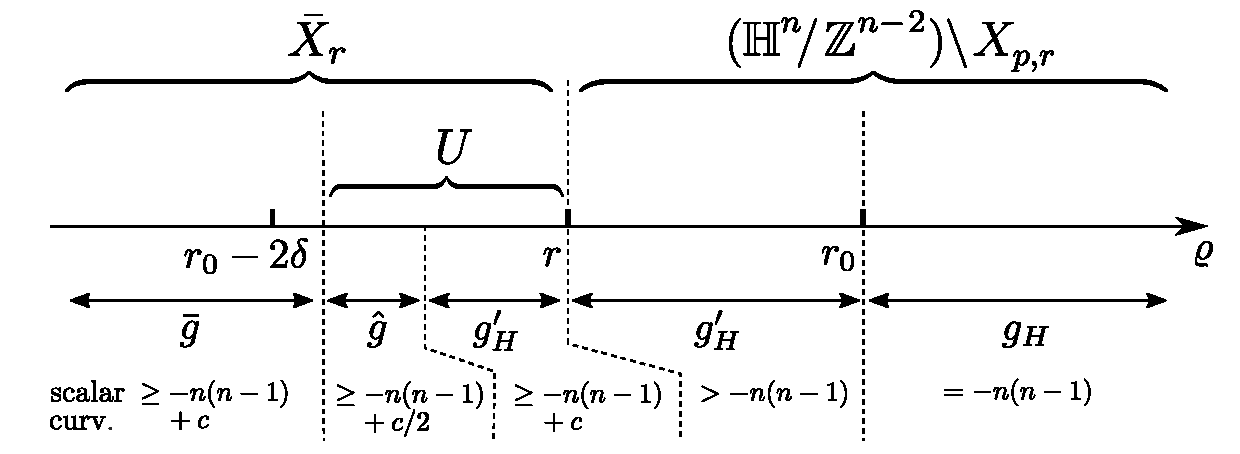
\includegraphics[scale = 0.5]{../assets/1168/Fig_gluingCstr.pdf}
	\caption{A schematic picture of $(\bs{M}, \bs{g})$.}\label{Fig_glue}
\end{figure}
\section*{Editable literal labels of original Figure1 (transcription)}
\noindent\textbf{Locator convention:} Original \texttt{Fig\_gluingCstr.pdf} stays unchanged. These are its printed labels, in panel order, without inferred numerical locations for its unnamed dividers.
\par\noindent Top braces, left to right: $\bar X_r$; $(\mathbb{H}^n/\mathbb{Z}^{n-2})\setminus X_{p,r}$. The inner bracket is $U$.
\par\noindent Axis arrow: $\varrho$. Named axis marks, left to right: $r_0-2\delta$; $r$; $r_0$.
\par\noindent Metric arrows, left to right: $\bar g$; $\hat g$; $g'_H$; $g'_H$; $g_H$.
\par\noindent The printed row heading is ``scalar curv.''. Its five region entries, left to right, are
\[
\begin{array}{ccccc}
\ge -n(n-1)+c & \ge -n(n-1)+c/2 & \ge -n(n-1)+c & > -n(n-1) & = -n(n-1).
\end{array}
\]
\noindent The braces, directed axis, double-ended metric arrows and unnamed dashed boundaries retain the original asset geometry. No new boundary value or derived curvature formula is added.

\begin{thebibliography}{99}
\bibitem[2]{ACG08}
Andersson L., Cai M., Galloway G.J., Rigidity and positivity of mass for
  asymptotically hyperbolic manifolds, \href{https://doi.org/10.1007/s00023-007-0348-2}{\textit{Ann. Henri Poincar\'e}}
  \textbf{9} (2008), 1--33, \href{https://arxiv.org/abs/math.DG/0703259}{arXiv:math.DG/0703259}.

\bibitem[8]{BMN2011}
Brendle S., Marques F.C., Neves A., Deformations of the hemisphere that
  increase scalar curvature, \href{https://doi.org/10.1007/s00222-010-0305-4}{\textit{Invent. Math.}} \textbf{185} (2011),
  175--197, \href{https://arxiv.org/abs/1004.3088}{arXiv:1004.3088}.

\bibitem[19]{Gr93}
Gromov M., Positive curvature, macroscopic dimension, spectral gaps and higher
  signatures, in Functional Analysis on the Eve of the 21st Century,
  {V}ol.~{II} ({N}ew {B}runswick, {NJ}, 1993), \textit{Progr. Math.}, Vol. 132,
  \href{https://doi.org/10.1007/s10107-010-0354-x}{Birkh\"auser}, Boston, MA, 1996, 1--213.

\bibitem[21]{Gr2019}
Gromov M., Scalar curvature of manifolds with boundaries: natural questions and
  artificial constructions, \href{https://arxiv.org/abs/1811.04311}{arXiv:1811.04311}.

\bibitem[22]{Gr2021}
Gromov M., Four lectures on scalar curvature, in Perspectives in Scalar
  Curvature. {V}ol.~1, Editors M.~Gromov, H.B. Lawson Jr., \href{https://doi.org/10.1007/10.1142/9789811273223_000}{World Scientific},
  Hackensack, NJ, 2023, 1--514, \href{https://arxiv.org/abs/1908.10612}{arXiv:1908.10612}.

\bibitem[23]{GL1983}
Gromov M., Lawson Jr. H.B., Positive scalar curvature and the {D}irac operator
  on complete {R}iemannian manifolds, \href{https://doi.org/10.1007/BF02953774}{\textit{Inst. Hautes \'Etudes Sci. Publ.
  Math.}} \textbf{1983} (1983), 83---196.

\bibitem[30]{MinOo89}
Min-Oo M., Scalar curvature rigidity of asymptotically hyperbolic spin
  manifolds, \href{https://doi.org/10.1007/BF01452046}{\textit{Math. Ann.}} \textbf{285} (1989), 527--539.

\bibitem[34]{SWW2022}
Shi Y., Wang W., Wei G., Total mean curvature of the boundary and nonnegative
  scalar curvature fill-ins, \href{https://doi.org/10.1515/crelle-2021-0072}{\textit{J.~Reine Angew. Math.}} \textbf{784}
  (2022), 215--250, \href{https://arxiv.org/abs/2007.06756}{arXiv:2007.06756}.

\end{thebibliography}
\end{document}
